\section*{Zadání}
Implementujte alespoň dvě rozdílné metody korelace souborů číselných dat [Correlation and dependence, Wikipedia]. Můžete uvažovat například Pearsonova korelační koeficient a Spearmanův koeficient pořadové korelace. Pro vybrané metody implementujte algoritmus v jazyce MATLAB. Následně metody korelace porovnejte na ilustrativním souboru dat (využijte databáze příkladů na Courseware).

\section*{O co jde?}
Při práci s větším objemem dat může být složité najít souvislost mezi jedním zdrojem dat a druhým zdrojem dat. V takovém případě se vyplatí využít algoritmů, do kterých vstupují hodnoty X a s nimi (možná) související hodnoty Y. Tyto algoritmy následně vrací informaci o míře korelace dat. Pokud např. hodnota X vždy vzroste o jasně daný přírůstek a hodnota Y na tento přírůstek zareaguje vždy stejnou odezvou, můžeme bezpečně prohlásit, že mezi těmito soubory dat existuje vzájemný vztah.

\begin{figure}[H]
    \centering
	\makebox[\textwidth]{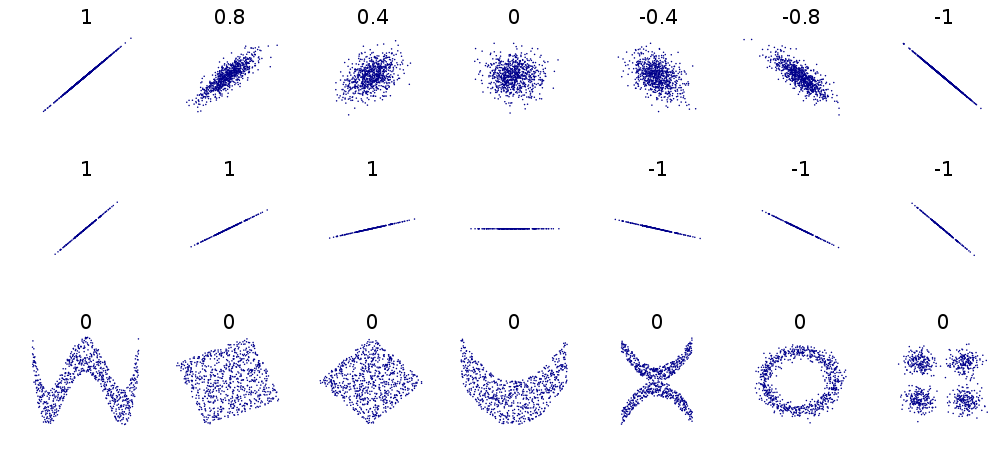
\includegraphics[width=\textwidth]{img/correlation.png}}
	\caption{Korelační koeficienty podle Pearsonova algoritmu}
	\label{fig:correlation}
\end{figure}

Na výše uvedeném obrázku je vidět přesně toto chování. Prostřední řádka ukazuje na perfektní korelaci - je jednoduché najít vztah mezi osou X a Y. U prvního řádku to již není vždy tak jednoznačné, nebo korelace vůbec neexistuje. Stejně tak neexistuje korelace v posledním řádku (nelze najít žádný jasný vztah mezi X a Y).

\section*{Popis korelačních algoritmů}
V této práci jsou implementovány dva algoritmy pro zjišťování korelace dat: Pearsonův korelační koeficient a Spearmanův koeficient pořadové korelace. Pearsonův korelační koeficient je roven $+1$ v případě ideální vzrůstající lineární závislosti dat a $-1$ v případě klesající lineární závislosti (nepřímá úměra). V ostatních případech se koeficient nachází v intervalu $(-1;+1)$ a popisuje míru korelace ($0$ = data nekorelují).

A protože každý kód, který nemá napsané testy, je spíše přání než-li skutečný kód, následují krátké unit testy, které testují výše uvedená pravidla a až poté následuje konkrétní implementace:

\begin{minted}[linenos]{matlab}
function testPearsonCorrelated(testCase)
    A = [1 2 3 4];
    B = [1 2 3 4]; % rho === 1.0
    testCase.verifyEqual(pearson(Correlation, A, B), 1.0);
end
\end{minted}

První parametr testovací funkce je aktuální hodnota, druhý parametr je potom očekávaná hodnota. Celá testovací sada lze spustit pomocí příkazu \texttt{run(CorrelationTest)}, jehož výstup by měl vypadat následovně (úspěšný průběh testů):

\begin{minted}[linenos]{text}
>> run(CorrelationTest)
Running CorrelationTest
.........
Done CorrelationTest
__________

Totals:
   9 Passed, 0 Failed, 0 Incomplete.
   0.14226 seconds testing time.
\end{minted}

To je důkaz, že všechny testy fungují. Podobně vypadá test pro klesající závislost (stále Pearson):

\begin{minted}[linenos]{matlab}
function testPearsonCorrelated(testCase)
    A = [1 2 3 4];
    B = [4 3 2 1]; % rho === -1.0
    testCase.verifyEqual(pearson(Correlation, A, B), -1.0);
end
\end{minted}

Toto chování lze popsat matematickým vzorcem pro výpočet Pearsonova korelačního koeficientu:

\begin{equation}
\rho_{X,Y} = corr(X,Y) = \frac{cov(X,Y)}{\sigma_X \cdot \sigma_Y}
\end{equation}

Kde $cov(X,Y)$ je kovariance hodnot $X$ a $Y$ a $\sigma$ značí směrodatnou odchylku. Samotný výpočet Pearsonova korelačního koeficientu je lze naprogramovat takto:

\begin{minted}[linenos]{matlab}
function rho = pearson(obj, X, Y)
    X = X(:); % vectorize
    Y = Y(:);
    covariance = cov(X, Y);
    rho = covariance(1, 2) / (std(X) * std(Y));
    if isnan(rho)
        error('pearson:undefined', 'Correlation coefficient
            is undefined because the variance of Y is zero.')
    end
end
\end{minted}

Prvně algoritmus vezme vstupující matice nebo vektory a vyrobí z nich jednu dlouhou posloupnost dat. Následně vypočítá Pearsonův koeficient korelace podle vzorce. Spearmanův koeficient pořadové korelace se chová velmi podobně pouze s tím rozdílem, že se hledá korelace nikoliv hodnot jako takových, ale jejich indexů (pořadí) v souboru dat. Implementace může vypadat třeba takto:

\begin{minted}[linenos]{matlab}
function rho = spearman(obj, X, Y)
    X = X(:); % vectorize
    Y = Y(:);
    [~, rankX] = sort(X); % calulate Spearman ranking
    [~, rankY] = sort(Y);
    rho = obj.pearson(rankX, rankY);
end
\end{minted}

Za povšimnutí stojí, že Spearmanův algoritmus využívá s výhodou Pearsonův (pouze vstupní hodnoty jsou indexy v původním souboru dat). Rozdíl mezi Pearsonovým a Spearmanovým algoritmem je dobře pochopitelný z tohoto testu:

\begin{minted}[linenos]{matlab}
function testNonlinearCorrelation(testCase)
    A = [0 10 101 102];
    B = [1 100 500 2000];
    testCase.verifyEqual(pearson(Correlation, A, B), 0.7544);
    testCase.verifyEqual(spearman(Correlation, A, B), 1.0);
end
\end{minted}

Zatímco Pearsonův koeficient je $0.7544$, tak Spearmanův je $1.0$. Proč? Person hledá korelaci vzhledem k lineárnímu charakteru souboru dat, Spearman však sleduje tendenci dat. Tzn. že pokud vzroste A, vzroste i B. Pokud opět vzroste A, opět vzroste B (nezáleží an velikosti přírůstku). Z toho plyne, že data korelují a z hlediska Spearmanova algoritmu korelují perfektně.

\section*{Korelace většího objemu dat}
Ačkoliv bylo v zadání dáno, že mám použít vzorové matice, nevěděl jsem si s tím rady. Pro ověření algoritmů je totiž zapotřebí dvou odlišných souborů dat o stejné velikosti, mezi kterými se hledá závislost a proto jsou přiložené matice nevhodné. Vytvořil jsem proto třídu \texttt{GenerateDemoData}, která k tomuto účelu slouží. Tato třída umí podle předem dané křivky vygenerovat sadu bodů s tím, že body jsou rozptýleny kolem křivky podle normálního rozdělení s určitou variabilitou. Takto může vypadat průběh vygenerovaných hodnot pro $y=x^3$ s vysokou variabilitou (červené hodnoty) a ten samý průběh pouze vynásobený $-1$ s menší variabilitou (modré hodnoty):

\begin{figure}[H]
    \centering
	\makebox[\textwidth]{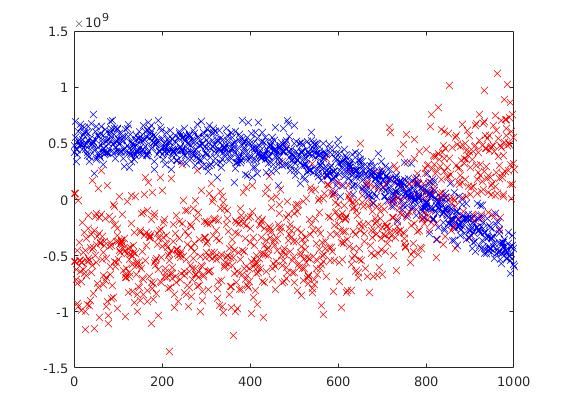
\includegraphics[width=\textwidth]{img/random.jpg}}
	\caption{Náhodně vygenerované hodnoty s variabilitou kolem daných křivek} %0.6378 a -0.8591
	\label{fig:random}
\end{figure}

V tomto případě vychází Pearsonův koeficient $0.6378$ (pro vzrůstající hodnoty) a $-0.8591$ pro klesající hodnoty. Spearmanův koeficient se v tomto případě téměř neliší. Z toho je vidět, že korelační koeficient se tím více blíží mezní hodnotě, čím jsou data méně rozptýlena (a tedy korelace dat je jasnější).

U velmi velkých matic je problém s paměťovou náročností. Algoritmus je napsán až příliš naivně a je schopen zabrat celou paměť. Přemýšlel jsem proto, jesli by bylo možné počítat Pearsonův korelační koeficient postupně. To však nejde. Proč ne? Důkaz mého tvrzení lze vyzkoušet takto:

\begin{minted}[linenos]{matlab}
Ax = [1 2 3 4 5 6 7 8 9 10];
Ay = [6 9 8 4 1 2 5 6 3 5];

Bx = [91 92 93 94 95 96 97 98 99 100];
By = [65 69 68 61 63 65 66 67 62 60];

c = Correlation(false);
c.pearson(Ax, Ay) % -0.4160
c.pearson(Bx, By) % -0.4973
\end{minted}

Pokud však vezmeme v úvahu celý soubor dat (tedy A i B dohromady), výsledek je zcela jiný:
\begin{minted}[linenos]{matlab}
Cx = [1 2 3 4 5 6 7 8 9 10 91 92 93 94 95 96 97 98 99 100];
Cy = [6 9 8 4 1 2 5 6 3 5 65 69 68 61 63 65 66 67 62 60];
c.pearson(Cx, Cy) % 0.9915
\end{minted}

Zatímco části souboru dat vycházejí záporně, celý soubor dat poukazuje (podle Pearsona) na velmi dobrou korelaci. Bylo by tedy zapotřebí zvolit méně naivní postup a vybírat podsoubory dat lépe (třeba z obou konců zároveň). Tuto otázku by bylo třeba řešit např. v případě paralelizace, to však není předmětem této práce.

\subsection*{Závěrem}
V této práci se řeší korelace dat, je však potřeba upozornit na to, že z korelace neplyne kauzalita. To že mezi soubory dat existuje určitá souvislost nutně neznamená (ale může znamenat), že změna jedné veličiny přímo způsobuje změnu druhé veličiny. Korelace je nutnou, nikoliv postačující podmínkou kauzality.

Dále je třeba si uvědomit, že výsledný korelační koeficient (zejména Pearsonův) nijak nevypovídá o rozložení testovaných bodů. Mohlo by se totiž zdát, že Pearsonův koeficient ukazuje míru linearity bodů, to však není pravda. Důkazem je test \texttt{testAnscombesQuartet}, který ukazuje čtyři sady bodů, které mají od linerity daleko a každý vypadá úplně jinak, přesto Pearsonův korelační koeficient vychází vždy stejně. Vizuální pohled na data může být tedy důležitý.

Z předchozího pozorování se tedy Spearmanův koeficient pořadové korelace jeví jako vhodnější protože není citlivý na hodnoty předloženého souboru dat, ale na jejich pořadí a tendenci. Nicméně jeho výpočet je náročnější, protože je potřeba zjistit pořadí prvků v souboru dat. Všechny naprogramované třídy jsou příloženy na následujích stránkách.

\newpage
\subsection*{Implementace korelačních algoritmů}
\begin{minted}[linenos]{matlab}
classdef Correlation
    properties (SetAccess = private)
        withGraphics;
    end

    methods
        function obj = Correlation(withGraphics) % constructor
            if nargin == 0
                withGraphics = false;
            end
            obj.withGraphics = withGraphics;
        end

        function rho = pearson(obj, X, Y)
            [X, Y] = obj.vectorize(X, Y);
            rho = obj.pearsonWithoutVectorize(X, Y);
        end

        function rho = spearman(obj, X, Y)
            [X, Y] = obj.vectorize(X, Y);
            [~, rankX] = sort(X); % calulate Spearman ranking
            [~, rankY] = sort(Y);
            rho = obj.pearsonWithoutVectorize(rankX, rankY);
        end
    end

    methods (Access = private)
        function [X, Y] = vectorize(obj, X, Y)
            X = X(:); Y = Y(:);
        end

        function rho = pearsonWithoutVectorize(obj, X, Y)
            covariance = cov(X, Y);
            rho = covariance(1, 2) / (std(X) * std(Y));
            if isnan(rho)
                error('pearson:undefined', 'Correlation coefficient
                    is undefined because the variance of Y is zero.')
            end
            if obj.withGraphics
                plotmatrix(X, Y)
            end
        end
    end
end

\end{minted}

\newpage
\subsection*{Pomocná třída pro generování dat}
\begin{minted}[linenos]{matlab}
classdef GenerateDemoData
    %GENERATEDEMODATA Class for generation demo data
    %   This class is quite pointless with stupid API, but it generates
    %   random data with value deviation around math curve and that's
    %   pretty useful for correlation testing.

    properties (SetAccess = private)
        length;
        deviationScale;
    end

    methods
        function obj = GenerateDemoData(length, deviationScale)
            if nargin == 0
                length = 1000;
                deviationScale = 1;
            end
            obj.length = length;
            obj.deviationScale = deviationScale;
        end

        function [X, Y] = exponential(obj)
            [X, Y] = obj.generateTable(@(x) x^3-0.5e9,
                obj.length * 3e5 * obj.deviationScale);
        end
        function [X, Y] = quadratic(obj)
            [X, Y] = obj.generateTable(@(x) -x^3+0.5e9,
                obj.length * 1e5 * obj.deviationScale);
        end
    end

    methods (Access = private)
        function value = randn(obj, mu, sigma)
            value = (randn * sigma) + mu;
        end

        function [X, Y] = generateTable(obj, func, deviation)
            for index = 1:obj.length
                X(index) = index;
                Y(index) = obj.randn(func(index), deviation);
            end
        end
    end

end
\end{minted}

\newpage
\subsection*{Testy korelačních algoritmů}
\begin{minted}[linenos]{matlab}
classdef CorrelationTest < matlab.unittest.TestCase
    % run(CorrelationTest)

    methods (Test)
        function testPearsonCorrelated(testCase)
            A = [1 2 3 4];
            B = [1 2 3 4];
            % actual, expected, ...
            testCase.verifyEqual(pearson(Correlation, A, B), 1.0,
                'AbsTol', 1e-15);
        end

        function testPearsonAnticorrelated(testCase)
            A = [1 2 3 4];
            B = [4 3 2 1];
            testCase.verifyEqual(pearson(Correlation, A, B), -1.0,
                'AbsTol', 1e-15);
        end

        function testPearsonWithoutCorrelation(testCase)
            A = [3 4 5 6];
            B = [1 1 1 1];
            testCase.verifyError(@() pearson(Correlation, A, B),
                'pearson:undefined', 'Correlation coefficient is
                 undefined because the variance of Y is zero.');
        end

        function testPearsonZeroCorrelation(testCase)
            A = [1 2 1 2];
            B = [1 1 2 2];
            testCase.verifyEqual(pearson(Correlation, A, B), 0.0);
            testCase.verifyEqual(spearman(Correlation, A, B), 0.8);
        end

        function testSpearmanHalfCorrelation(testCase)
            % Spearman should be 0.5 but Kendall shoul be 1.0
            A = [1 2 3];
            B = [1 3 2];
            testCase.verifyEqual(pearson(Correlation, A, B), 0.5);
            testCase.verifyEqual(spearman(Correlation, A, B), 0.5);
        end

        function testNonlinearCorrelation(testCase)
            A = [0 10 101 102];
            B = [1 100 500 2000];
            testCase.verifyEqual(pearson(Correlation, A, B), 0.7544,
                'AbsTol', 1e-4);
            testCase.verifyEqual(spearman(Correlation, A, B), 1.0,
                'AbsTol', 1e-15);
        end

        function testUniformlyRandomCorrelation(testCase)
            c = Correlation(false); % without graphics (default)
            A = randi(100, 100); % uniformly distributed pseudorandom integers
            B = randi(100, 100);
            testCase.verifyEqual(pearson(c, A, B), 0.05, 'RelTol', 10);
            testCase.verifyEqual(spearman(c, A, B), 0.05, 'RelTol', 10);
        end

        function testLargeDemoData(testCase)
            g = GenerateDemoData(1000, 1);
            [X, Y] = g.exponential();
            [A, B] = g.quadratic();
            c = Correlation(false);
            testCase.verifyEqual(pearson(c, X, Y), 0.6, 'RelTol', 10);
            testCase.verifyEqual(pearson(c, A, B), -0.8, 'RelTol', 10);
        end

        function testAnscombesQuartet(testCase)
            % https://en.wikipedia.org/wiki/Anscombe%27s_quartet
            c = Correlation(false);
            test = @(x, y) testCase.verifyEqual(pearson(c, x, y), 0.816,
                'RelTol', 0.001);
            X1 = [10 8 13 9 11 14 6 4 12 7 5];
            Y1 = [8.04 6.95 7.58 8.81 8.33 9.96 7.24 4.26 10.84 4.82 5.68];
            test(X1, Y1);
            X2 = [10 8 13 9 11 14 6 4 12 7 5];
            Y2 = [9.14 8.14 8.74 8.77 9.26 8.10 6.13 3.10 9.13 7.26 4.74];
            test(X2, Y2);
            X3 = [10 8 13 9 11 14 6 4 12 7 5];
            Y3 = [7.46 6.77 12.74 7.11 7.81 8.84 6.08 5.39 8.15 6.42 5.73];
            test(X3, Y3);
            X4 = [8 8 8 8 8 8 8 19 8 8 8];
            Y4 = [6.58 5.76 7.71 8.84 8.47 7.04 5.25 12.50 5.56 7.91 6.89];
            test(X4, Y4);
        end
    end

end
\end{minted}
